\documentclass[UTF8,AutoFakeBold]{szu2024}


\renewcommand{\titleCN}{基于xx分析}
\renewcommand{\titleEN}{Analysis Based on xx}


% 文本
\usepackage{ctex}
\usepackage{fancyhdr}

% dgq package
\usepackage{makecell}


%圆
%\usepackage{xeCJK}

%%adding package 边距设置
\usepackage[left=31.7mm,right=31.7mm,top=25.4mm,bottom=25.4mm]{geometry}
\usepackage{titlesec}

\usepackage{setspace} %使用调整行距的包
\usepackage{subfigure,floatrow}
\usepackage{url}
\usepackage{caption}
\usepackage{subcaption}
\usepackage{caption,cite,amsbsy,amsmath,amsfonts,multirow,color,array,booktabs,colortbl}
\usepackage{algorithm}
\usepackage{algorithmic}
\usepackage{pdfpages}
\usepackage{changepage}


% \usepackage{algorithmicx,algorithm}
\usepackage{epsfig,bm}
\usepackage{slashbox}
\usepackage{enumitem}
\usepackage{amssymb,amsthm,amssymb}
\usepackage{graphicx,subfigure}
\usepackage{graphicx}
\usepackage{ulem}
\usepackage{floatrow}
\usepackage{arydshln} % 加载arydshln宏包
\usepackage{tabularx}
\floatsetup[table]{capposition=top}
\floatsetup[figure]{capposition=bottom}
\newfloatcommand{capbtabboxTable}{table}[][\FBwidth]
\newfloatcommand{capbtabboxFigure}{figure}[][\FBwidth]
\newcommand{\norm}[1]{\left\lVert #1 \right\rVert}


% 重新调整参考文献项目之间的行距
\usepackage{bibspacing}
\setlength{\bibspacing}{1\baselineskip}

%给目录和参考文献加上超链接
\usepackage[hidelinks]{hyperref}

%引用
\newcommand{\upcite}[1]{{\textsuperscript{\cite{#1}}}}

%defines the height of the header
% \setlength{\headheight}{15pt}
\setlength{\headheight}{23pt}
\setlength{\headsep}{7.25mm}


\hypersetup{
    pdfborder = {0 0 0} 
}

%document begin
\begin{document}

%封面 自行配置生成pdf文件导入即可
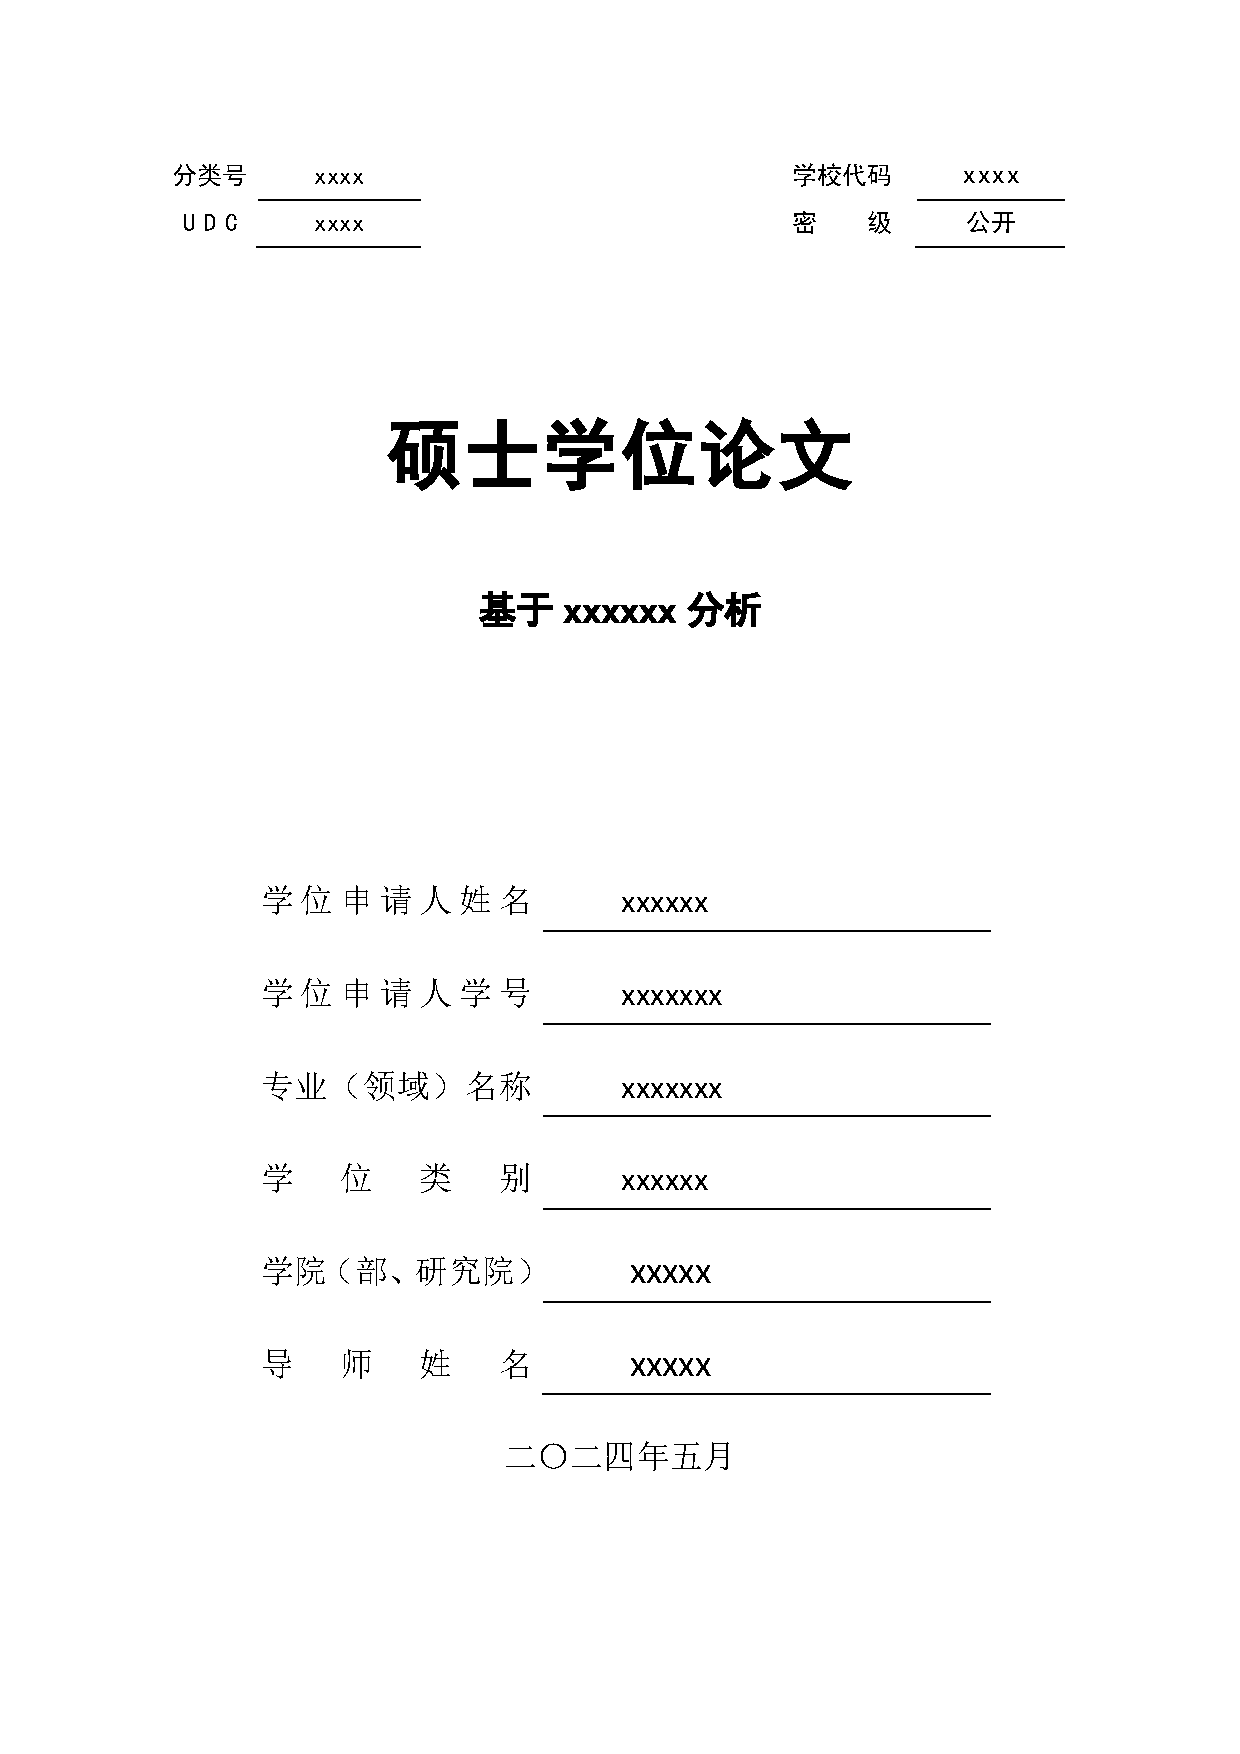
\includepdf[pages={1,2}]{chapter/masterPage.pdf}

%中英文摘要 以及 缩写表
\begin{abstractCN}
\setlength{\baselineskip}{23pt} %设置行距23磅


研究生生活是一段充满智慧和探索的旅程。在这个阶段,学生们接触到更深层次的学术内容,面对更具挑战性的问题,并在学术界展开独立研究。研究生院的学术氛围让学生们有机会深入研究他们感兴趣的领域,与导师和同行们共同探讨和解决复杂的问题。

除了学术挑战,研究生生活也涵盖了更广泛的社交和职业发展。学生们与来自不同背景和领域的同学共同学习,建立起深厚的人际关系。同时,与导师的交流和合作为学生们提供了更广泛的职业发展机会,帮助他们在未来的职业生涯中更好地发展。

在研究生院,学生们有机会参与各种学术和社会活动,拓展他们的视野。这包括学术研讨会、专题讲座、学术合作项目等。通过这些活动,他们能够更全面地了解自己的专业领域,并与其他研究者建立联系。


\end{abstractCN}


\begin{keywordCN}
xx分析;xx学习
\end{keywordCN}

\begin{abstractEN}
\setlength{\baselineskip}{23pt} %设置行距23磅
Graduate life is a journey filled with wisdom and exploration. During this stage, students delve into more profound academic content, face more challenging problems, and embark on independent research within the academic community. The academic atmosphere in graduate school provides students with opportunities to deeply explore their areas of interest, engaging in discussions and solving complex problems collaboratively with mentors and peers.

Beyond academic challenges, graduate life encompasses a broader spectrum of social and professional development. Students learn from and connect with peers from diverse backgrounds and fields, fostering profound interpersonal relationships. Simultaneously, interactions and collaborations with mentors open up broader opportunities for professional development, aiding students in shaping their future careers more effectively.

In graduate school, students have the chance to participate in various academic and social activities, broadening their horizons. This includes academic seminars, special lectures, collaborative research projects, and more. Through these activities, they gain a comprehensive understanding of their respective fields and establish connections with other researchers.
\end{abstractEN}

\begin{keywordEN}
xx Analysis; xx Learning
\end{keywordEN}



\begin{signAndABC}

\begin{adjustwidth}{-\leftskip}{0pt}
 % 调整表格宽度
\renewcommand\arraystretch{1.5}
\begin{tabular}{l@{\hspace{4em}}l}
VAE & 变分自编码器(Variational Auto-Encoder) \\
CNN & 卷积神经网络(Convolutional Neural Network) \\
\end{tabular}
\end{adjustwidth}


\end{signAndABC}


 

\setlength{\baselineskip}{23pt} %设置行距23磅

\tableofcontents	%目录

%%%%%%%%% 图索引和表索引
% \renewcommand\listfigurename{\songti\zihao{2}{\textbf{图~~目~~录}}}
% \renewcommand\listtablename{\songti\zihao{2}{\textbf{表~~目~~录}}}

% \renewcommand{\figurename}{图}
% \renewcommand{\tablename}{表}

\makeatletter %
\@addtoreset{equation}{section}
\makeatother  %
\renewcommand\theequation{{\thesection}%
				.{\arabic{equation}}}
%%%%%%%%%% 表每节重新标号
\makeatletter %
\@addtoreset{table}{section}
\makeatother  %
\renewcommand{\thetable}{\thesection-\arabic{table}}
\captionsetup[table]{labelsep=space, labelfont=bf}
%%%%%%%% 图每节重新标号
\makeatletter %
\@addtoreset{figure}{section}
\makeatother  %
\renewcommand{\thefigure}{\thesection-\arabic{figure}}
\captionsetup[figure]{labelsep=space, labelfont=bf}
%labelfont=normalfont}
% subfigure重新编号\ref
\makeatletter
\renewcommand{\p@subfigure}{\thefigure}
\makeatother


%adding chapters 1-5 从1开始计数
\setcounter{page}{1}

\clearpage

\section{绪论}

\subsection{研究背景及意义}
研究生生活是一段充满智慧和探索的旅程。在这个阶段,学生们接触到更深层次的学术内容,面对更具挑战性的问题,并在学术界展开独立研究。研究生院的学术氛围让学生们有机会深入研究他们感兴趣的领域,与导师和同行们共同探讨和解决复杂的问题。

除了学术挑战,研究生生活也涵盖了更广泛的社交和职业发展。学生们与来自不同背景和领域的同学共同学习,建立起深厚的人际关系。同时,与导师的交流和合作为学生们提供了更广泛的职业发展机会,帮助他们在未来的职业生涯中更好地发展。

在研究生院,学生们有机会参与各种学术和社会活动,拓展他们的视野。这包括学术研讨会、专题讲座、学术合作项目等。通过这些活动,他们能够更全面地了解自己的专业领域,并与其他研究者建立联系。

%图片 pdf格式 测试
如图\ref{fig:w-xxx}所示

 \begin{figure}[h]
    \centering

\includegraphics[width=0.8\textwidth]{figure/cp1/xxx.pdf}
     \caption{11111}  
     \label{fig:w-xxx}
 \end{figure}


如表\ref{tab:xxx}所示

% 表格测试 input插入
\begin{table*}[t]
  \centering
  \renewcommand\arraystretch{1.4}
  \caption{评估结果}
    %\resizebox{0.\textwidth}{!}{
    \begin{tabular}{l@{\hspace{4em}}c@{\hspace{4em}}c@{\hspace{4em}}c}
    \toprule
    模型 & F1 & F2 & F3  \\
    \midrule
AE & xx	 & 0.111 &	0.111 
   \\
VAE &\textbf{0.222} &	0.312 &	0.44 
 \\
    \bottomrule
    \end{tabular}%
    %}
  \label{tab:xxx}%
\end{table*}%










\subsection{研究背景及意义}
研究生生活是一段充满智慧和探索的旅程。在这个阶段,学生们接触到更深层次的学术内容,面对更具挑战性的问题,并在学术界展开独立研究。研究生院的学术氛围让学生们有机会深入研究他们感兴趣的领域,与导师和同行们共同探讨和解决复杂的问题。

除了学术挑战,研究生生活也涵盖了更广泛的社交和职业发展。学生们与来自不同背景和领域的同学共同学习,建立起深厚的人际关系。同时,与导师的交流和合作为学生们提供了更广泛的职业发展机会,帮助他们在未来的职业生涯中更好地发展。

在研究生院,学生们有机会参与各种学术和社会活动,拓展他们的视野。这包括学术研讨会、专题讲座、学术合作项目等。通过这些活动,他们能够更全面地了解自己的专业领域,并与其他研究者建立联系。
\clearpage

\section{xxxxxxx}

\subsection{引言}

\subsubsection{研究问题表述}
研究生生活是一段充满智慧和探索的旅程。在这个阶段,学生们接触到更深层次的学术内容,面对更具挑战性的问题,并在学术界展开独立研究。研究生院的学术氛围让学生们有机会深入研究他们感兴趣的领域,与导师和同行们共同探讨和解决复杂的问题\upcite{cryer2011}。

除了学术挑战,研究生生活也涵盖了更广泛的社交和职业发展。学生们与来自不同背景和领域的同学共同学习,建立起深厚的人际关系。同时,与导师的交流和合作为学生们提供了更广泛的职业发展机会,帮助他们在未来的职业生涯中更好地发展。

在研究生院,学生们有机会参与各种学术和社会活动,拓展他们的视野。这包括学术研讨会、专题讲座、学术合作项目等。通过这些活动,他们能够更全面地了解自己的专业领域,并与其他研究者建立联系。
\subsubsection{研究问题表述}
研究生生活是一段充满智慧和探索的旅程。在这个阶段,学生们接触到更深层次的学术内容,面对更具挑战性的问题,并在学术界展开独立研究。研究生院的学术氛围让学生们有机会深入研究他们感兴趣的领域,与导师和同行们共同探讨和解决复杂的问题。

除了学术挑战,研究生生活也涵盖了更广泛的社交和职业发展。学生们与来自不同背景和领域的同学共同学习,建立起深厚的人际关系。同时,与导师的交流和合作为学生们提供了更广泛的职业发展机会,帮助他们在未来的职业生涯中更好地发展。

在研究生院,学生们有机会参与各种学术和社会活动,拓展他们的视野。这包括学术研讨会、专题讲座、学术合作项目等。通过这些活动,他们能够更全面地了解自己的专业领域,并与其他研究者建立联系\upcite{atamuradov2017prognostics}。

\subsection{引言}

\subsubsection{研究问题表述}
研究生生活是一段充满智慧和探索的旅程。在这个阶段,学生们接触到更深层次的学术内容,面对更具挑战性的问题,并在学术界展开独立研究。研究生院的学术氛围让学生们有机会深入研究他们感兴趣的领域,与导师和同行们共同探讨和解决复杂的问题。

除了学术挑战,研究生生活也涵盖了更广泛的社交和职业发展。学生们与来自不同背景和领域的同学共同学习,建立起深厚的人际关系。同时,与导师的交流和合作为学生们提供了更广泛的职业发展机会,帮助他们在未来的职业生涯中更好地发展。

在研究生院,学生们有机会参与各种学术和社会活动,拓展他们的视野。这包括学术研讨会、专题讲座、学术合作项目等。通过这些活动,他们能够更全面地了解自己的专业领域,并与其他研究者建立联系。

\subsubsection{研究问题表述}

研究生生活是一段充满智慧和探索的旅程。在这个阶段,学生们接触到更深层次的学术内容,面对更具挑战性的问题,并在学术界展开独立研究。研究生院的学术氛围让学生们有机会深入研究他们感兴趣的领域,与导师和同行们共同探讨和解决复杂的问题。

除了学术挑战,研究生生活也涵盖了更广泛的社交和职业发展。学生们与来自不同背景和领域的同学共同学习,建立起深厚的人际关系。同时,与导师的交流和合作为学生们提供了更广泛的职业发展机会,帮助他们在未来的职业生涯中更好地发展。

在研究生院,学生们有机会参与各种学术和社会活动,拓展他们的视野。这包括学术研讨会、专题讲座、学术合作项目等。通过这些活动,他们能够更全面地了解自己的专业领域,并与其他研究者建立联系。
\clearpage

\section{xxxxxxx}

\subsection{引言}

\subsubsection{研究问题表述}
研究生生活是一段充满智慧和探索的旅程。在这个阶段,学生们接触到更深层次的学术内容,面对更具挑战性的问题,并在学术界展开独立研究。研究生院的学术氛围让学生们有机会深入研究他们感兴趣的领域,与导师和同行们共同探讨和解决复杂的问题\upcite{cryer2011}。

除了学术挑战,研究生生活也涵盖了更广泛的社交和职业发展。学生们与来自不同背景和领域的同学共同学习,建立起深厚的人际关系。同时,与导师的交流和合作为学生们提供了更广泛的职业发展机会,帮助他们在未来的职业生涯中更好地发展。

在研究生院,学生们有机会参与各种学术和社会活动,拓展他们的视野。这包括学术研讨会、专题讲座、学术合作项目等。通过这些活动,他们能够更全面地了解自己的专业领域,并与其他研究者建立联系。
\subsubsection{研究问题表述}
研究生生活是一段充满智慧和探索的旅程。在这个阶段,学生们接触到更深层次的学术内容,面对更具挑战性的问题,并在学术界展开独立研究。研究生院的学术氛围让学生们有机会深入研究他们感兴趣的领域,与导师和同行们共同探讨和解决复杂的问题。

除了学术挑战,研究生生活也涵盖了更广泛的社交和职业发展。学生们与来自不同背景和领域的同学共同学习,建立起深厚的人际关系。同时,与导师的交流和合作为学生们提供了更广泛的职业发展机会,帮助他们在未来的职业生涯中更好地发展。

在研究生院,学生们有机会参与各种学术和社会活动,拓展他们的视野。这包括学术研讨会、专题讲座、学术合作项目等。通过这些活动,他们能够更全面地了解自己的专业领域,并与其他研究者建立联系\upcite{atamuradov2017prognostics}。

\subsection{引言}

\subsubsection{研究问题表述}
研究生生活是一段充满智慧和探索的旅程。在这个阶段,学生们接触到更深层次的学术内容,面对更具挑战性的问题,并在学术界展开独立研究。研究生院的学术氛围让学生们有机会深入研究他们感兴趣的领域,与导师和同行们共同探讨和解决复杂的问题。

除了学术挑战,研究生生活也涵盖了更广泛的社交和职业发展。学生们与来自不同背景和领域的同学共同学习,建立起深厚的人际关系。同时,与导师的交流和合作为学生们提供了更广泛的职业发展机会,帮助他们在未来的职业生涯中更好地发展。

在研究生院,学生们有机会参与各种学术和社会活动,拓展他们的视野。这包括学术研讨会、专题讲座、学术合作项目等。通过这些活动,他们能够更全面地了解自己的专业领域,并与其他研究者建立联系。

\subsubsection{研究问题表述}

研究生生活是一段充满智慧和探索的旅程。在这个阶段,学生们接触到更深层次的学术内容,面对更具挑战性的问题,并在学术界展开独立研究。研究生院的学术氛围让学生们有机会深入研究他们感兴趣的领域,与导师和同行们共同探讨和解决复杂的问题。

除了学术挑战,研究生生活也涵盖了更广泛的社交和职业发展。学生们与来自不同背景和领域的同学共同学习,建立起深厚的人际关系。同时,与导师的交流和合作为学生们提供了更广泛的职业发展机会,帮助他们在未来的职业生涯中更好地发展。

在研究生院,学生们有机会参与各种学术和社会活动,拓展他们的视野。这包括学术研讨会、专题讲座、学术合作项目等。通过这些活动,他们能够更全面地了解自己的专业领域,并与其他研究者建立联系。
\clearpage

\section{xxxxxxx}

\subsection{引言}

\subsubsection{研究问题表述}
研究生生活是一段充满智慧和探索的旅程。在这个阶段,学生们接触到更深层次的学术内容,面对更具挑战性的问题,并在学术界展开独立研究。研究生院的学术氛围让学生们有机会深入研究他们感兴趣的领域,与导师和同行们共同探讨和解决复杂的问题\upcite{cryer2011}。

除了学术挑战,研究生生活也涵盖了更广泛的社交和职业发展。学生们与来自不同背景和领域的同学共同学习,建立起深厚的人际关系。同时,与导师的交流和合作为学生们提供了更广泛的职业发展机会,帮助他们在未来的职业生涯中更好地发展。

在研究生院,学生们有机会参与各种学术和社会活动,拓展他们的视野。这包括学术研讨会、专题讲座、学术合作项目等。通过这些活动,他们能够更全面地了解自己的专业领域,并与其他研究者建立联系。
\subsubsection{研究问题表述}
研究生生活是一段充满智慧和探索的旅程。在这个阶段,学生们接触到更深层次的学术内容,面对更具挑战性的问题,并在学术界展开独立研究。研究生院的学术氛围让学生们有机会深入研究他们感兴趣的领域,与导师和同行们共同探讨和解决复杂的问题。

除了学术挑战,研究生生活也涵盖了更广泛的社交和职业发展。学生们与来自不同背景和领域的同学共同学习,建立起深厚的人际关系。同时,与导师的交流和合作为学生们提供了更广泛的职业发展机会,帮助他们在未来的职业生涯中更好地发展。

在研究生院,学生们有机会参与各种学术和社会活动,拓展他们的视野。这包括学术研讨会、专题讲座、学术合作项目等。通过这些活动,他们能够更全面地了解自己的专业领域,并与其他研究者建立联系\upcite{atamuradov2017prognostics}。

\subsection{引言}

\subsubsection{研究问题表述}
研究生生活是一段充满智慧和探索的旅程。在这个阶段,学生们接触到更深层次的学术内容,面对更具挑战性的问题,并在学术界展开独立研究。研究生院的学术氛围让学生们有机会深入研究他们感兴趣的领域,与导师和同行们共同探讨和解决复杂的问题。

除了学术挑战,研究生生活也涵盖了更广泛的社交和职业发展。学生们与来自不同背景和领域的同学共同学习,建立起深厚的人际关系。同时,与导师的交流和合作为学生们提供了更广泛的职业发展机会,帮助他们在未来的职业生涯中更好地发展。

在研究生院,学生们有机会参与各种学术和社会活动,拓展他们的视野。这包括学术研讨会、专题讲座、学术合作项目等。通过这些活动,他们能够更全面地了解自己的专业领域,并与其他研究者建立联系。

\subsubsection{研究问题表述}

研究生生活是一段充满智慧和探索的旅程。在这个阶段,学生们接触到更深层次的学术内容,面对更具挑战性的问题,并在学术界展开独立研究。研究生院的学术氛围让学生们有机会深入研究他们感兴趣的领域,与导师和同行们共同探讨和解决复杂的问题。

除了学术挑战,研究生生活也涵盖了更广泛的社交和职业发展。学生们与来自不同背景和领域的同学共同学习,建立起深厚的人际关系。同时,与导师的交流和合作为学生们提供了更广泛的职业发展机会,帮助他们在未来的职业生涯中更好地发展。

在研究生院,学生们有机会参与各种学术和社会活动,拓展他们的视野。这包括学术研讨会、专题讲座、学术合作项目等。通过这些活动,他们能够更全面地了解自己的专业领域,并与其他研究者建立联系。
\clearpage


\section{总结与展望}

\subsection{论文总结}
xxx


\subsection{研究展望}
xxxxx


\clearpage
%参考文献
\fancyhead{}
\fancyhead[C]{\songti\zihao{5}{参考文献}}
\fancyfoot[C]{\songti\zihao{5}{\thepage}}

\begin{spacing}{1.8}
	\bibliographystyle{gbt7714-2005} 
	\bibliography{ref_paper}
\end{spacing}



\clearpage
\fancyhead{}
\fancyhead[C]{\songti\zihao{5}{致谢}}
\fancyfoot[C]{\songti\zihao{5}{\thepage}}
\begin{szuAppendix}{致~谢}

\songti\zihao{5}
\setlength{\baselineskip}{23pt}

感谢

\end{szuAppendix}



\clearpage
\fancyhead{}
\fancyhead[C]{\songti\zihao{5}{攻读硕士学位期间学术成果}}
\fancyfoot[C]{\songti\zihao{5}{\thepage}}
\begin{szuAppendixB}{攻读硕士学位期间的研究成果}
% \begin{spacing}{1.5}
\songti\zihao{5}
\setlength{\baselineskip}{15pt}
   

\noindent{\heiti\zihao{-3}{学术论文}}

\vspace{0.3\baselineskip} 

\noindent{[1]~ \textbf{xxxx}, xxxx, xxxx. xxxx.(SCI收录,对应学位论文第三章)}


    % \noindent{
    % [2]~ ***, ***, ***, ***, \textbf{***}. xxxxxx[J].xxxxx, 2022, 252: 109310.(SCI一区,第四作者) }
    
\end{szuAppendixB}


\end{document}

%当需要在论文末尾插入相关的文件,可以生成pdf文件格式进行附加,附加一页就是1,多页就是1,2,3
%\includepdf[pages={1}]{chapter/comment.pdf}
%\includepdf[pages={1}]{chapter/decision.pdf}

